\documentclass[letterpaper,12pt]{article}
\usepackage[utf8]{inputenc}
\usepackage{fullpage}
\usepackage{courier}
\usepackage[margin=0.75in]{geometry}
\usepackage{listings}
\usepackage{color}
\usepackage{graphicx}
\usepackage[width=5in]{caption}
\usepackage{hyphenat}
\usepackage{hyperref}
\usepackage{float}
\usepackage{multirow}

% Format a sectionless paragraph
\newcommand*\unparagraph{
	\par
	\nopagebreak
	\vskip3.25ex plus1ex minus.2ex
	\noindent
}

% define extra colors
\definecolor{dkgreen}{rgb}{0,0.6,0}
\definecolor{purple}{RGB}{159,0,197}

% define the code listing format
\lstset{
	language=C++,
	basicstyle=\footnotesize\ttfamily,
	backgroundcolor=\color{white},
	showspaces=false,
	showstringspaces=false,
	frame=none,
	tabsize=3,
	keywordstyle=\color{purple},
	commentstyle=\color{dkgreen},
	stringstyle=\color{blue},
	escapeinside={\%*}{*)}
}

% efine the title/header
\title{\Large CS 3468\\Lab 4} 
\author{Jared Wallace}
\date{}

\begin{document}

\maketitle

\vspace{30mm}

\section*{Objectives}
\begin{enumerate}
\item Learn to use a sensor to sense the environment
\item Learn to read and analyze sensing data
\end{enumerate}

\section*{Tasks}
\subsection*{Sense Light}
\begin{enumerate}
    \item Besides communication, sensing is the other major function of a sensor.
          Depending on the actual hardware components, a sensor may sense light,
          temperature, presence of a magnetic field, humidity, sound, acceleration,
          etc. The diagram below shows a sensor application that senses the light
          level once per second.
        \begin{figure}[H]
            \centering
            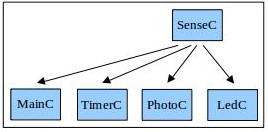
\includegraphics[width=4in]{diagram1.jpg}
        \end{figure}
         The application has seven components in total, and the component
         PhotoC is what actually handles the sensing of light levels.
        \begin{itemize}
            \item System component MainC
            \item System component new TimerMilliC() as TimerC
            \item System component PhotoC
            \item System component LedC
            \item Application component SenseC
        \end{itemize}
    \item Now, open the API link \url{http://www.tinyos.net/tinyos-2.x/doc/nesdoc/micaz/}.
          Find the API documents of the first five system components and their
          interfaces. Implement a sensor application such that:
          \begin{itemize}
            \item The sensor senses the light every 2 seconds.
            \item The red LED lights up when the application is sensing.
            \item The green LED indicates that the intensity of the light
                  is beyond a certain threshold (0x180).
            \item The yellow LED indicates that the intensity of the light is
                  below a certain threshold (0x180).
            \item The lab instructor will give you a threshold to use as a
                  reference. You may need to adjust the threshold according
                  to your environment.
          \end{itemize}
    \item Compile and run your application, and show your lab instructor
\end{enumerate}
\subsection*{Send data back to the computer}
\begin{enumerate}
    \item Now, use the radio transmission component (like we did previously) to
          send the data back to a base station connected to the computer.
    \item The application should have the following work flow:
        \begin{itemize}
            \item The sensor samples the light intensity every 2 seconds.
            \item The sensor computes an average of the light intensity
                  measured every 6 seconds, and sends that average back
                  to the base station.
            \item The red LED should light up to indicate when it is sensing.
                  It should be off when the data is being transmitted out.
            \item The green LED should light to indicate that the intensity of
                  the light is beyond a certain threshold (0x180).
            \item The yellow LED should light to indicate that the intensity
                  of the light is below a certain threshold (0x180).
        \end{itemize}
    \item Follow the lab instructors example, and run a Java program to read
          and display the data being sent back. Demonstrate your application for
          the lab instructor.
\end{enumerate}
\subsection*{Model the sensor and the environment}
\begin{enumerate}
    \item The lab instructor will turn off the lights in the room, and give you
        a set of simple calibration tools.
    \item Your sensor measures the intensity of the background light.
        Read and record three sets of received data in Table 1.
        If the deviation is more than 10 percent of the average,
        please redo the measurement.
        \begin{table}[H]
        \begin{center}
            \begin{tabular}{|c|c|c|c|c|}
                \hline
                \textbf{Data 1} & \textbf{Data 2} & \textbf{Data 3} & \textbf{Average} & \textbf{Deviation} \\ \hline
                 & & & & \\ \hline
            \end{tabular}
        \end{center}
        \end{table}
    \item Turn on a light source and move it around your sensor.
        Measure the light intensity at various positions. Read and record three
        data measurements at each position, and record them in the following table.
        If the deviation is more than 10 percent of the average, please redo
        the measurements.
        \begin{table}[H]
        \begin{center}
            \begin{tabular}{|c|c|c|c|c|c|c|}
                \hline
                \textbf{Angle} & \textbf{Distance (ft)} & \textbf{Data 1} & \textbf{Data 2} & \textbf{Data 3} & \textbf{Average} & \textbf{Deviation} \\ \hline
                \multirow{5}{*}{0} & 0.5 & & & & & \\ \cline{2-7}
                & 1.0 & & & & & \\ \cline{2-7}
                & 1.5 & & & & & \\ \cline{2-7}
                & 2.0 & & & & & \\ \cline{2-7}
                & 3.0 & & & & & \\ \hline
                \multirow{5}{*}{30} & 0.5 & & & & & \\ \cline{2-7}
                & 1.0 & & & & & \\ \cline{2-7}
                & 1.5 & & & & & \\ \cline{2-7}
                & 2.0 & & & & & \\ \cline{2-7}
                & 3.0 & & & & & \\ \hline
                \multirow{5}{*}{60} & 0.5 & & & & & \\ \cline{2-7}
                & 1.0 & & & & & \\ \cline{2-7}
                & 1.5 & & & & & \\ \cline{2-7}
                & 2.0 & & & & & \\ \cline{2-7}
                & 3.0 & & & & & \\ \hline
                \multirow{5}{*}{90} & 0.5 & & & & & \\ \cline{2-7}
                & 1.0 & & & & & \\ \cline{2-7}
                & 1.5 & & & & & \\ \cline{2-7}
                & 2.0 & & & & & \\ \cline{2-7}
                & 3.0 & & & & & \\ \hline
            \end{tabular}
        \end{center}
        \end{table}
\end{enumerate}
\section*{Lab Report}
\begin{enumerate}
   \item Please demonstrate your program to the lab instructor and let him check your code at the end of the current lab project.
   \item Your project report is due at the beginning of the next lab.
   \item Grading criteria
      \begin{itemize}
         \item Demonstration, 15 percent
         \item Code, 15 percent
         \item Report, 70 percent
      \end{itemize}
\end{enumerate}
\section*{Report instructions}
Format:
\begin{enumerate}
   \item Include your name and ID in the first page
   \item Font size of at least 10pt
   \item Single spaced
   \item Maximum of 5 pages (I will take points off for exceeding this without any good reason)
   \item Please submit as PDF online, and turn in a hard copy
\end{enumerate}
Content:
\begin{enumerate}
   \item Introduction (10 percent of the report grade) Please summarize the task of this lab and what you have learned in the lab
   \item Implementation (30 percent of the report grade) Please describe in detail how your made your program. Show what components you used, how they are wired, and through what interfaces.
   \item Experiment (30 percent of the report grade) Please describe in detail what can be observed from your program and explain how said observed behavior is a result of your code (and not happy coincidence).
\end{enumerate}

% Comic at the bottom
\begin{figure}[ht!]
	\centering
	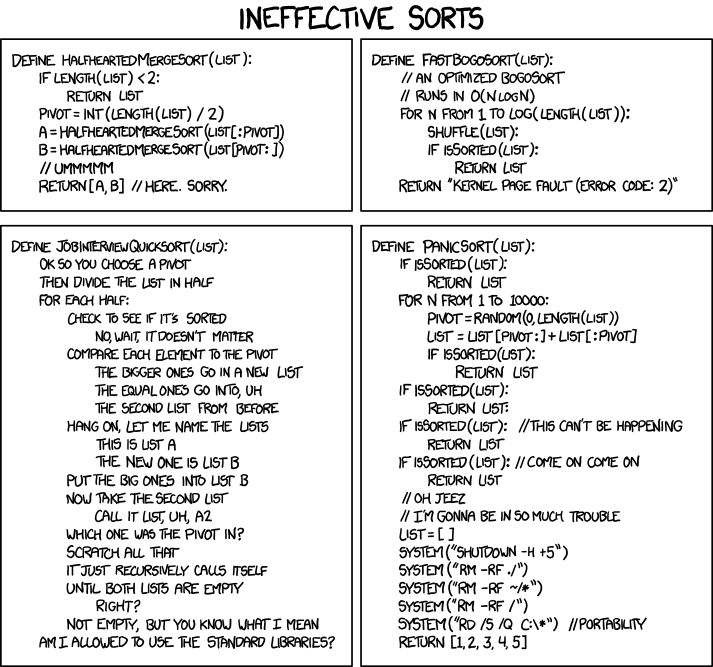
\includegraphics[width=4in]{ineffective_sorts.png}
    \caption*{StackSort connects to StackOverflow, searches for 'sort a list', and downloads and runs code snippets until the list is sorted.}
\end{figure}

\end{document}
